\section{Results}
\label{sec:results}

\subsection{Readout: strong for chat-model text, weak for base-model text}
\label{sec:readout}

\begin{figure}[t]
\centering
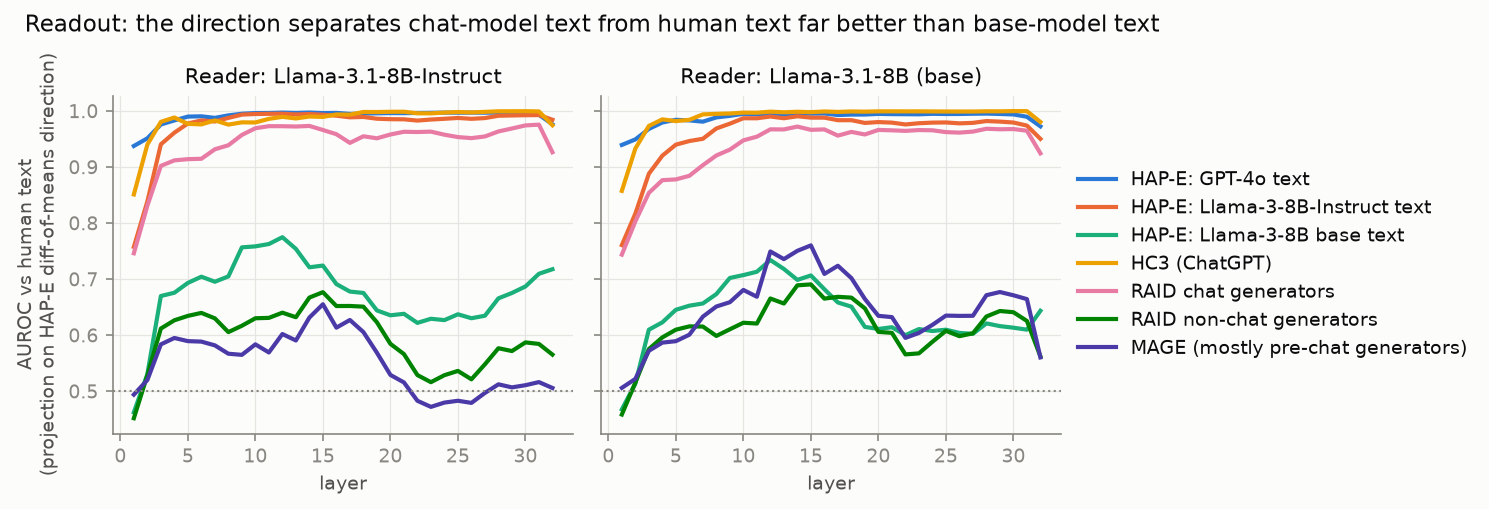
\includegraphics[width=0.95\linewidth]{figures/fig1_readout_by_layer.png}
\caption{AUROC of the projection on the \hape difference-of-means direction against human text, by layer and reading model. The direction separates chat-model text from human text almost perfectly from the early layers on and transfers to \hcthree and \raid chat generators. Text from base and pre-chat generators stays far lower at every layer.}
\label{fig:readout}
\end{figure}

\begin{table}[t]
\centering
\caption{Readout at layer 12: AUROC of the projection on \airead against human text. Rows in bold are generators that are not chat-tuned.}
\label{tab:readout}
\begin{tabular}{@{}lcc@{}}
\toprule
Test set & Instruct reader & Base reader \\
\midrule
\hape held-out, chat generators (diff-of-means / LR probe) & 0.996 / 1.000 & 0.991 / 0.999 \\
\hape GPT-4o text & 0.997 & 0.995 \\
\hape Llama-3-8B-Instruct text & 0.995 & 0.990 \\
{\bf \hape Llama-3-8B base text} & {\bf 0.775} & {\bf 0.734} \\
{\bf \hape Llama-3-70B base text} & {\bf 0.750} & {\bf 0.702} \\
\hcthree (ChatGPT vs.\ human answers) & 0.990 & 0.999 \\
\raid chat generators & 0.973 & 0.967 \\
{\bf \raid non-chat generators} & {\bf 0.640} & {\bf 0.665} \\
{\bf \mage (mostly pre-chat generators)} & {\bf 0.602} & {\bf 0.749} \\
Leave-one-genre-out, \hape (min--max over 6 genres) & 0.981--1.000 & 0.969--1.000 \\
\bottomrule
\end{tabular}
\end{table}

\Figref{fig:readout} and \tabref{tab:readout} reproduce the transferable direction of the probe literature.
\airead separates held-out chat-model text from human text at AUROC 0.996, holds up when a genre is left out (0.981--1.000), and transfers to \hcthree (0.990) and \raid chat generators (0.973).
Directions fitted on \hcthree and \raid reach 0.971 and 0.993 on \hape.

The same direction is weak for text that a model wrote without chat tuning: 0.75--0.78 for Llama-3 base text, 0.64 for \raid non-chat generators and 0.60 for \mage.
In human-SD units along the direction, chat-model texts sit at 4.4--4.8 and base-model texts at 1.0--1.1.
This is not an artifact of which generators were in the fit: a direction fitted on GPT-4o text only separates Llama-instruct text at 0.990 and Llama-base text at 0.674.
H1 therefore holds for chat-model text and fails as a statement about machine authorship.
The logistic-regression probe reads out slightly better and has cosine only 0.39 with \airead.

\subsection{Causal test: specific but partial}
\label{sec:causal}

\begin{figure}[t]
\centering
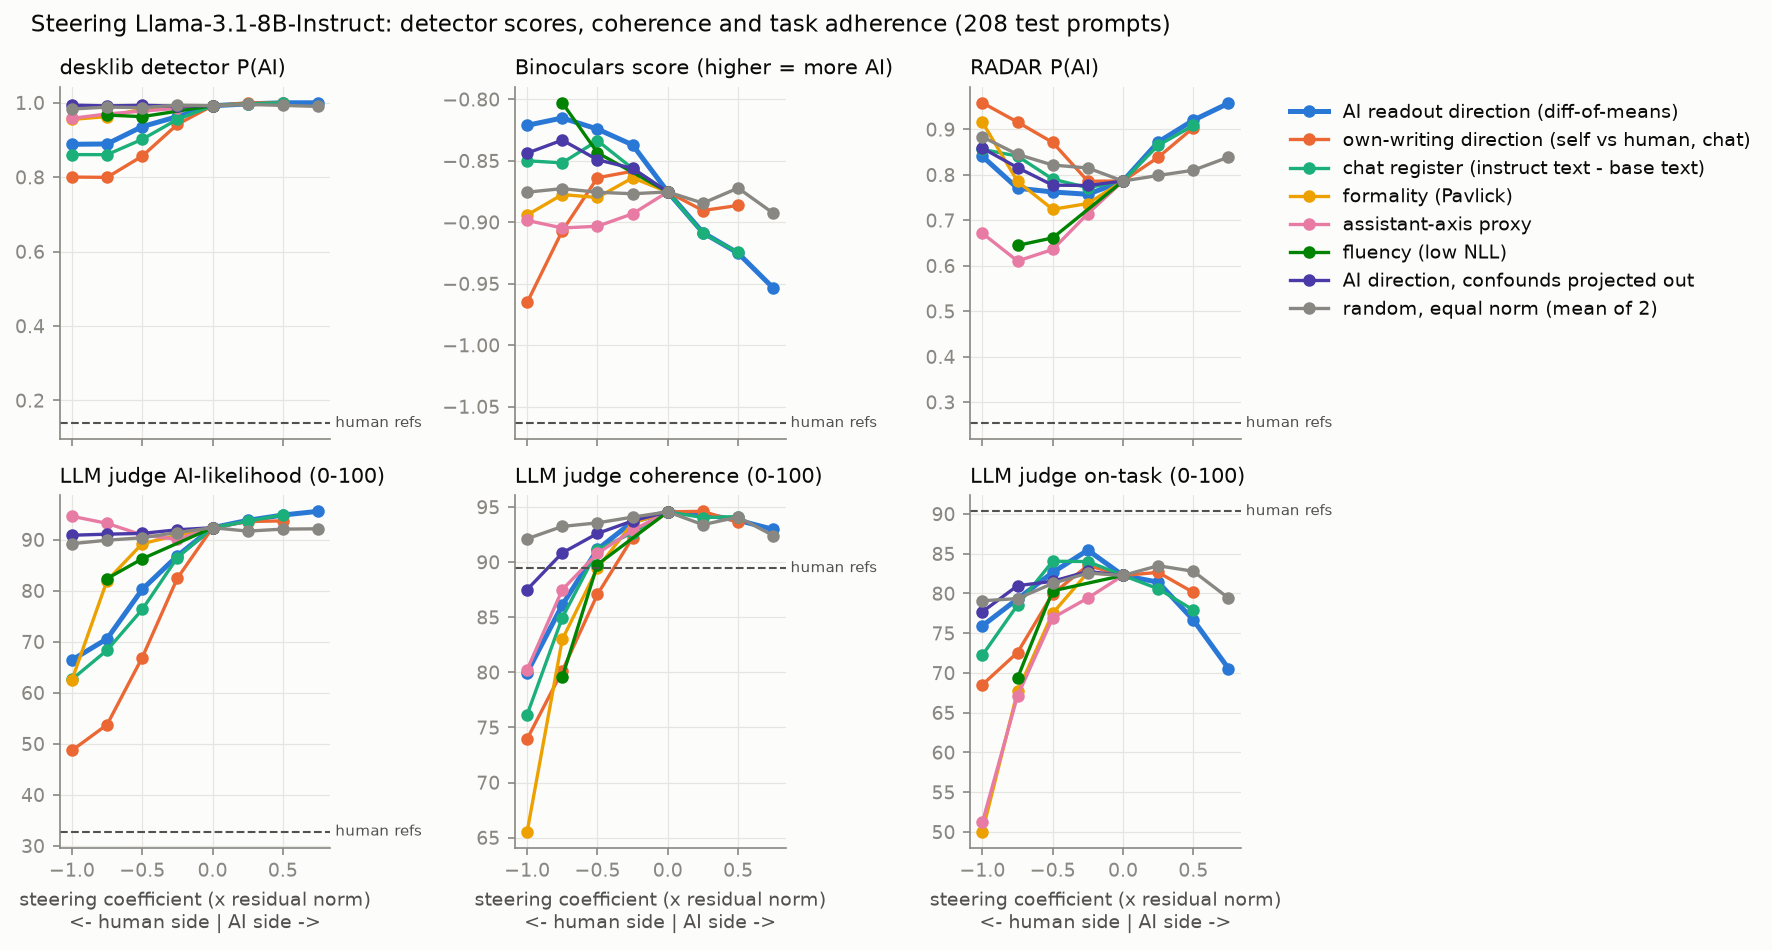
\includegraphics[width=\linewidth]{figures/fig3_dose_response.png}
\caption{Dose-response of steering \llamai at layer 12 on 208 test prompts. Negative coefficients steer toward the human side. The AI readout direction, the own-writing direction and the chat-register direction lower the judge's AI-likelihood and the \desklib score; the equal-norm random directions and the direction with confounds projected out do not. The \bino-style score moves the opposite way. Dashed lines mark human references.}
\label{fig:dose}
\end{figure}

\begin{table}[t]
\centering
\caption{Main steering results on 208 test prompts (layer 12). ``Flag'' is the share of texts above the 5\%-FPR threshold (\%). ``Sim'' is the embedding cosine with the unsteered output; ``RB'' is readback in human-SD units. Bold rows are the matched-coherence operating points of \airead and \writechat.}
\label{tab:main}
\resizebox{\textwidth}{!}{
\begin{tabular}{@{}lrcccccccccccc@{}}
\toprule
& & \multicolumn{2}{c}{Judge} & \multicolumn{2}{c}{\desklib} & \bino & \radar & \multicolumn{5}{c}{Quality and content} & \\
\cmidrule(lr){3-4}\cmidrule(lr){5-6}\cmidrule(lr){7-7}\cmidrule(lr){8-8}\cmidrule(lr){9-13}
Condition & $c$ & AI & flag & score & flag & flag & score & coher. & on-task & NLL & dist-3 & sim & RB \\
\midrule
Human references & & 32.8 & 3 & 0.139 & 5 & 5 & 0.25 & 89.4 & 90.3 & 2.68 & 0.99 & -- & 0.54 \\
Unsteered & & 92.4 & 99 & 0.992 & 100 & 83 & 0.79 & 94.6 & 82.3 & 1.48 & 0.98 & 1.00 & 4.35 \\
Unsteered, other seed & & 91.6 & 97 & 0.984 & 99 & 80 & 0.82 & 94.7 & 81.9 & 1.53 & 0.98 & 0.78 & 4.40 \\
Prompt ``write like a human'' & & 89.1 & 90 & 0.993 & 100 & 89 & 0.74 & 93.5 & 80.7 & 1.56 & 0.98 & 0.75 & 4.04 \\
Prompt ``write like an AI'' & & 94.2 & 100 & 0.997 & 100 & 75 & 0.84 & 94.4 & 80.6 & 1.47 & 0.98 & 0.80 & 5.05 \\
\midrule
\airead & $-0.25$ & 86.8 & 85 & 0.963 & 96 & 86 & 0.76 & 93.7 & 85.5 & 1.57 & 0.97 & 0.77 & 3.39 \\
\airead & $-0.50$ & 80.3 & 63 & 0.936 & 94 & 81 & 0.76 & 91.2 & 82.6 & 1.67 & 0.93 & 0.72 & 2.54 \\
{\bf \airead} & $\mathbf{-0.75}$ & {\bf 70.6} & {\bf 41} & {\bf 0.889} & {\bf 85} & {\bf 87} & {\bf 0.77} & {\bf 86.1} & {\bf 79.3} & {\bf 1.79} & {\bf 0.89} & {\bf 0.65} & {\bf 1.55} \\
\airead & $-1.00$ & 66.4 & 33 & 0.888 & 86 & 87 & 0.84 & 80.0 & 75.9 & 1.88 & 0.85 & 0.62 & 1.03 \\
\airead & $+0.25$ & 93.8 & 99 & 0.997 & 100 & 69 & 0.87 & 94.3 & 81.4 & 1.47 & 0.99 & 0.80 & 5.29 \\
\airead & $+0.50$ & 94.8 & 100 & 1.000 & 100 & 61 & 0.92 & 93.8 & 76.7 & 1.47 & 0.99 & 0.78 & 6.09 \\
\airead & $+0.75$ & 95.6 & 100 & 1.000 & 100 & 49 & 0.96 & 93.0 & 70.6 & 1.53 & 0.99 & 0.75 & 6.83 \\
\airead ablated, all layers & & 74.0 & 44 & 0.889 & 85 & 94 & 0.78 & 86.2 & 82.1 & 1.72 & 0.89 & 0.69 & 1.39 \\
\midrule
\writechat & $-0.25$ & 82.5 & 69 & 0.942 & 92 & 76 & 0.79 & 92.2 & 83.5 & 1.78 & 0.97 & 0.74 & 3.14 \\
{\bf \writechat} & $\mathbf{-0.50}$ & {\bf 66.9} & {\bf 35} & {\bf 0.857} & {\bf 82} & {\bf 76} & {\bf 0.87} & {\bf 87.1} & {\bf 79.9} & {\bf 2.16} & {\bf 0.94} & {\bf 0.65} & {\bf 1.70} \\
\writechat & $-0.75$ & 53.8 & 13 & 0.800 & 71 & 66 & 0.92 & 80.1 & 72.6 & 2.43 & 0.91 & 0.57 & 0.93 \\
\writechat ablated & & 65.7 & 26 & 0.764 & 69 & 86 & 0.75 & 83.6 & 81.4 & 2.14 & 0.93 & 0.68 & 1.34 \\
\ailr (probe weights) & $-0.75$ & 78.1 & 58 & 0.922 & 89 & 77 & 0.81 & 92.0 & 82.9 & 1.80 & 0.97 & 0.69 & 2.78 \\
\midrule
\dir{random0} & $-0.75$ & 91.5 & 95 & 0.995 & 100 & 81 & 0.85 & 93.3 & 81.2 & 1.49 & 0.97 & 0.78 & 4.37 \\
\dir{random0} & $-1.00$ & 90.7 & 94 & 0.987 & 99 & 78 & 0.90 & 92.5 & 80.0 & 1.54 & 0.97 & 0.77 & 4.33 \\
\dir{random1} & $-0.75$ & 88.3 & 87 & 0.982 & 99 & 75 & 0.84 & 93.2 & 77.5 & 1.69 & 0.98 & 0.72 & 4.02 \\
\dir{random0} ablated & & 91.1 & 95 & 0.994 & 100 & 79 & 0.81 & 93.7 & 82.3 & 1.49 & 0.98 & 0.81 & 4.44 \\
\bottomrule
\end{tabular}}
\end{table}

\Figref{fig:dose} and \tabref{tab:main} give the main run.

\para{What holds.}
{\em Dose-response in both signs.} Judge AI-likelihood, \desklib and readback fall monotonically with negative coefficients and rise with positive ones where there is headroom.
{\em Specificity.} Against the mean of the two random directions at the same coefficient, \airead at $c=-0.75$ changes the judge by $-19.3$ points (95\% CI $-22.8$ to $-15.7$) and \desklib by $-0.099$ ($-0.126$ to $-0.074$), both with Holm-corrected $p < 0.001$.
{\em Matched coherence.} \airead reaches $c=-0.75$ (coherence 86.1, on-task 79.3) with 41\% flagged by the judge and 85\% by \desklib. \writechat reaches $c=-0.5$ (coherence 87.1) with 35\% and 82\%. Random directions reach $c=-1.0$ with 85--94\% and 98--99\% (\figref{fig:frontier}).
{\em Better than prompting.} The ``write like a human'' prompt moves the judge by 3.3 points (CI 2.3--4.3) and does not move \desklib.
{\em Ablation.} Removing the direction at all layers gives judge 74.0 and \desklib flag 85\%; removing a random direction changes nothing.
{\em Closed loop.} Text written under steering re-reads at 1.55 SD, down from 4.35, so the intervention writes into the text the feature that the probe reads. Random steering leaves readback at 4.0--4.4.
{\em Not a length effect.} Steered outputs are shorter (140 to 117 words at $c=-0.75$). Truncating the unsteered outputs to the steered word counts leaves \desklib at 0.987 (steered: 0.889) and, on the 72 prompts judged before we reached an API limit, the judge at 93.0 (steered: 79.9 on the same prompts).
The effect is similar across tasks: $-22$, $-20$ and $-23$ judge points for \hape continuation, \hcthree answers and \raid writing.

\begin{figure}[t]
\centering
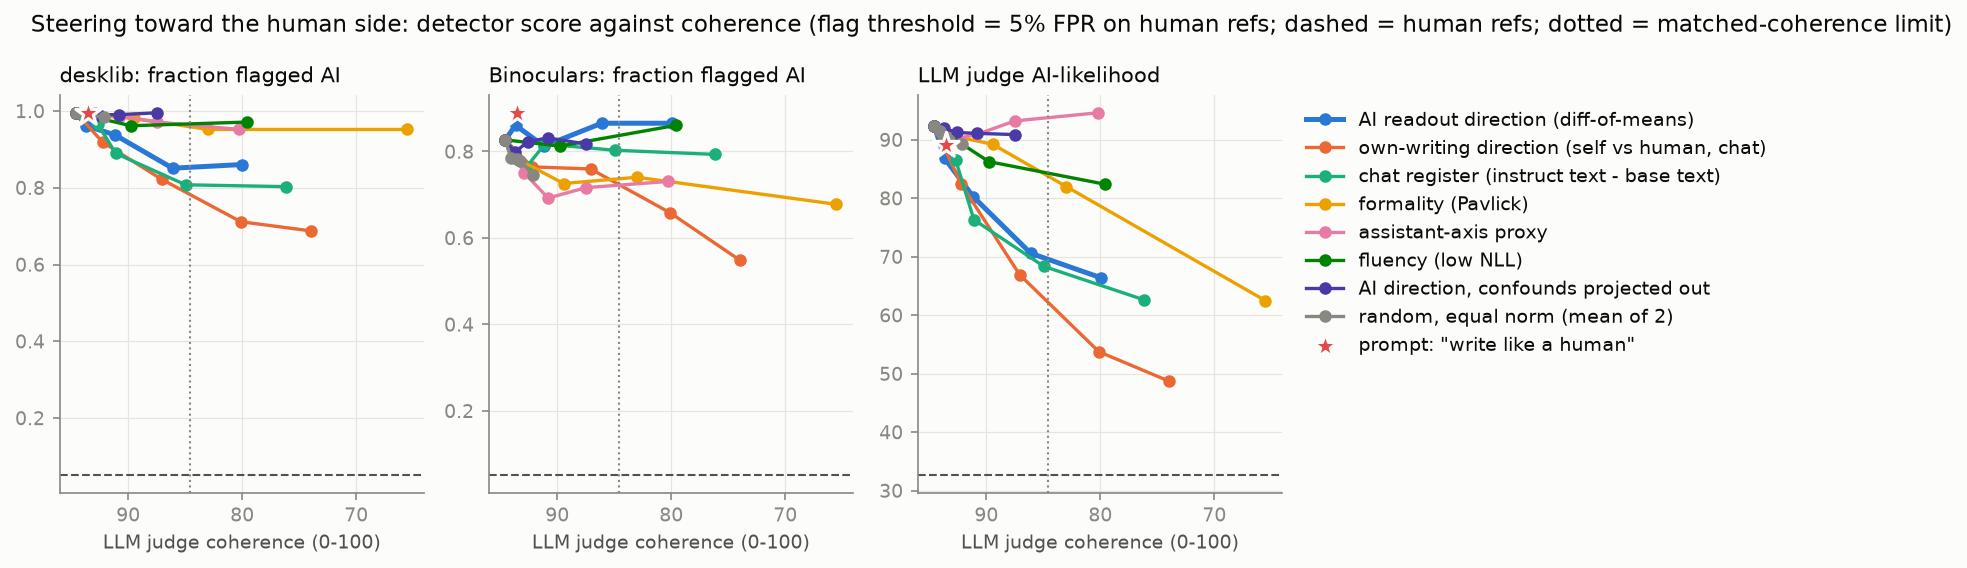
\includegraphics[width=\linewidth]{figures/fig4_frontier.png}
\caption{Detector score against judge coherence when steering toward the human side. Each line traces one direction over increasing $|c|$. The dotted line is the matched-coherence limit and the dashed line the human references. Only the AI readout, own-writing and chat-register directions lower the judge and \desklib before coherence is lost, and no direction comes near the human references on \desklib or \bino.}
\label{fig:frontier}
\end{figure}

\para{What does not hold.}
{\em Detector agreement.} \bino moves the wrong way: $+0.057$ against random at $c=-0.75$ (Holm $p<0.001$; 87\% flagged) and $-0.061$ at $c=+0.75$ (49\% flagged).
Over all 13{,}312 generated texts its Spearman correlation with the judge is $-0.24$ and with \desklib $-0.16$, although it separates unsteered output from human text at AUROC 0.93.
\radar does not differ from random on the human side (Holm $p = 0.60$).
The \hcthree RoBERTa score drops with steering (0.78 to 0.58), but the truncation control drops it as far (0.63), so we do not count it as evidence.
{\em Size.} At matched coherence the shift covers 37\% of the distance from unsteered output to human references on the judge and 12\% on \desklib. External NLL moves from 1.48 to 1.79, against 2.68 for human text.
{\em Content and quality.} Embedding similarity to the unsteered output falls from the seed-noise level of 0.78 to 0.65, distinct-3 falls from 0.98 to 0.89, and coherence drops 8.5 points. The output stays on task (79.3 vs.\ 82.3), but content is not held fixed.
{\em Positive side.} Steering toward AI lowers on-task scores (82.3 to 70.6 at $c=+0.75$) with coherence intact: on continuation prompts the model drifts into polished generic prose.

H2 is therefore partly supported: the direction is causal for how AI-like the text reads to a judge and, weakly, to the best supervised detector, but not for ``detected as AI'' in general.
\Tabref{tab:examples} shows typical outputs. Steered text is plainer and more colloquial, and its typical failure is looping.

\para{Readers vs.\ writers.}
The reading-derived direction controls writing, but less efficiently than the direction fitted on the model's own writing (\writechat: judge 66.9 at coherence 87.1, against 70.6 at 86.1).
The logistic-regression probe, the best reader, moves the judge least per unit norm among the three but preserves coherence best (78.1 at 92.0), in line with \citet{marks2023geometry}. We ran \ailr at two coefficients only, so its frontier is incomplete.

\begin{table}[t]
\centering
\caption{First lines of outputs for a \raid prompt asking for an IMDb review of {\em Vertigo}; the last row is a \hape fiction continuation that shows the typical failure (looping).}
\label{tab:examples}
\small
\begin{tabular}{@{}p{0.19\linewidth}p{0.77\linewidth}@{}}
\toprule
Condition & Output \\
\midrule
Unsteered & ``Alfred Hitchcock's `Vertigo' is a masterclass in suspense and psychological complexity. Released in 1958, this gripping thriller has stood the test of time\ldots'' \\
\airead, $c=-0.75$ & ``I just watched Vertigo for the third time and I still don't get it. I'm not saying that's a bad thing, I'm just saying that's what it's like. It's a masterful film by master filmmaker Alfred Hitchcock. He makes you think you know what's going on, then\ldots'' \\
\airead ablated & ``This is a very complex movie and I'm still not sure I completely understand it. The main character is a retired police officer who is a acrophobic (he is afraid of heights)\ldots'' \\
\airead, $c=+0.75$ & ``\ldots a masterclass in psychological suspense, weaving a complex web of obsession and deception that continues to captivate audiences to this day.'' \\
\airead, $c=-0.75$ (fiction) & ``It was a great comfort to him to be able to say with his eyes shut that the Lord had kept him from having a crop this year. It was a great comfort to him to be able to say that the Lord had kept him from having a crop next year\ldots'' \\
\bottomrule
\end{tabular}
\end{table}

\subsection{Disentanglement: the direction is chat register}
\label{sec:distinct}

\begin{figure}[t]
\centering
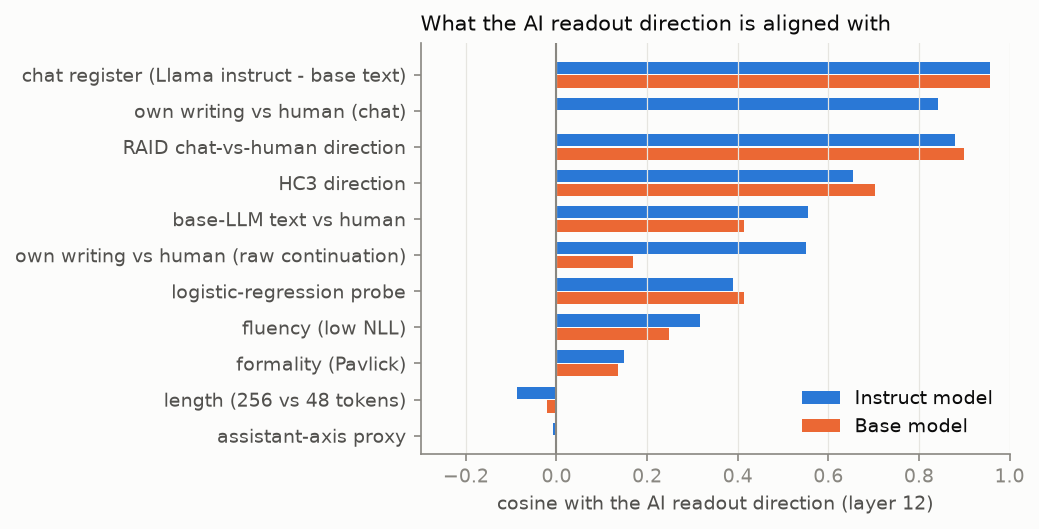
\includegraphics[width=0.8\linewidth]{figures/fig2_cosines.png}
\caption{Cosine of each candidate direction with the AI readout direction at layer 12, in both models. Chat register is almost parallel to it; formality, length and the assistant-axis proxy are close to orthogonal.}
\label{fig:cosines}
\end{figure}

\begin{table}[t]
\centering
\caption{Geometry at layer 12 of the instruct model. ``AUROC after removal'' is the held-out human-vs-chat AUROC after projecting the candidate out of the activations and refitting. ``Share removed'' is the share of \airead inside the candidate's span.}
\label{tab:geometry}
\resizebox{\textwidth}{!}{
\begin{tabular}{@{}lccc@{}}
\toprule
Candidate & Cosine with \airead & AUROC after removal & Share removed \\
\midrule
Chat register (Llama instruct $-$ base text) & {\bf 0.96} & {\bf 0.918} & {\bf 92\%} \\
Chat register, disjoint generators & 0.88 / 0.89 & -- & -- \\
Own writing vs.\ human, chat (\writechat) & 0.84 & -- & -- \\
Base-LLM text vs.\ human (\aibase) & 0.55 & -- & -- \\
Fluency (low NLL) & 0.32 & 0.996 & 10\% \\
Formality & 0.15 & 0.996 & 2\% \\
Length & $-0.09$ & 0.996 & 1\% \\
Assistant-axis proxy & $-0.01$ & 0.996 & $<0.1$\% \\
Genre subspace (5-D) & -- & 0.996 & 19\% \\
All of the above together & -- & 0.863 & 93\% \\
\bottomrule
\end{tabular}}
\end{table}

\para{Geometry.}
\Figref{fig:cosines} and \tabref{tab:geometry} show that \airead has cosine 0.96 with \chatreg, and that chat register accounts for 92\% of it.
The two directions share Llama-instruct texts, which inflates the cosine; with \airead fitted on GPT-4o text only and the register direction on the Llama 8B or 70B pair, it is 0.88--0.89.
Every other candidate is far from parallel: fluency 0.32, formality 0.15, length $-0.09$, assistant-axis proxy $-0.01$.
Projecting any of these out of the activations leaves the held-out AUROC at 0.996; projecting chat register out lowers it to 0.918.

Simple covariates do not explain the projection either.
The formality direction separates formal from informal sentences at AUROC 0.955 and human from AI text at 0.63, while \airead separates formal from informal sentences at 0.62.
NLL alone separates human from chat-model text at 0.89, but after regressing NLL and genre out of the projection, the projection still separates them at 0.957.
The Biber features \citep{biber1988variation} that correlate most with the projection are mean word length, nominalisations, prepositions, attributive adjectives and present participles (positive), and contractions, demonstrative pronouns, adverbs, second-person pronouns and emphatics (negative).
The same features order {\em human} texts along the direction ($r$ up to 0.60 and $-0.57$), so the direction is a property of the prose, with human text spread along it.

\begin{table}[t]
\centering
\caption{Steering with the candidate directions at equal norm (208 test prompts). Only directions that contain the chat-register component reproduce the effect of \airead on the judge and \desklib. ``Form.'' is the formality classifier score.}
\label{tab:candidates}
\resizebox{\textwidth}{!}{
\begin{tabular}{@{}lrccccccc@{}}
\toprule
Direction & $c$ & Judge AI & \desklib flag & \bino flag & Coher. & On-task & Form. & Readback \\
\midrule
Unsteered & & 92.4 & 100 & 83 & 94.6 & 82.3 & 0.81 & 4.35 \\
\airead & $-0.75$ & 70.6 & 85 & 87 & 86.1 & 79.3 & 0.81 & 1.55 \\
\chatreg & $-0.75$ & {\bf 68.4} & 81 & 80 & 85.0 & 78.5 & 0.86 & {\bf 1.28} \\
\midrule
\formality & $-0.50$ & 89.2 & 98 & 73 & 89.5 & 77.5 & 0.67 & 3.90 \\
\formality & $-0.75$ & 82.0 & 95 & 74 & 83.0 & 67.7 & 0.58 & 3.27 \\
\formality ablated & & 92.5 & 100 & 71 & 92.9 & 81.6 & 0.82 & 4.32 \\
\asstaxis & $-0.50$ & 90.9 & 99 & 69 & 90.8 & 76.9 & 0.72 & 4.40 \\
\asstaxis & $-0.75$ & 93.2 & 97 & 72 & 87.5 & 67.1 & 0.66 & 4.77 \\
\fluency & $-0.50$ & 86.3 & 96 & 81 & 89.8 & 80.3 & 0.65 & 3.43 \\
\lengthdir & $-0.50$ & 92.8 & 100 & 76 & 92.9 & 80.2 & 0.83 & 4.77 \\
\midrule
\perpall & $-1.00$ & 90.9 & 100 & 82 & 87.5 & 77.7 & 0.74 & 3.65 \\
\perppersona & $-0.75$ & 90.7 & 98 & 80 & 89.9 & 79.7 & 0.70 & 3.87 \\
\midrule
\aibase & $-0.75$ & 79.8 & {\bf 74} & {\bf 58} & 87.8 & 84.4 & 0.76 & 2.63 \\
\aihc & $-0.50$ & 72.1 & {\bf 74} & 73 & 88.4 & 82.6 & 0.76 & 2.32 \\
\bottomrule
\end{tabular}}
\end{table}

\para{Steering with the candidates.}
\Tabref{tab:candidates} gives the causal counterpart.
{\bf Formality is not it.} Steering toward informal lowers the formality classifier score (0.81 to 0.58), but the judge moves only when coherence collapses (at $c=-1.0$: judge 62.5 with coherence 65.5 and on-task 50.0). \airead leaves the formality score unchanged.
{\bf The assistant-axis proxy is not it.} Moving away from the assistant pole leaves the judge at 91--95 and \desklib unchanged while on-task falls to 51 at $c=-1.0$. It does lower \radar (0.79 to 0.61).
{\bf Chat register is it.} \chatreg steers like \airead (judge 68.4, \desklib flag 81\%). With the chat-register span removed (\perppersona, \perpall), the direction does nothing to the judge or \desklib, even at $c=-1.0$.

H3 is therefore refuted for chat register and supported for formality, fluency, length, genre and the assistant-axis proxy.

\para{A second axis.}
\aibase (base-LLM text minus human text; cosine 0.55 with \airead) is the only direction that lowers the \bino flag rate (83\% to 58\%), and it raises external NLL the most (2.35).
It also lowers \desklib more than \airead at similar coherence.
This is one run of one direction, and we did not test what it encodes.
\aihc, fitted on the confounded \hcthree contrast, also moves the judge and \desklib more than \airead at similar coherence, but it mixes register with whatever else separates Reddit answers from ChatGPT answers, so we cannot attribute its effect.

\subsection{Base vs.\ instruct: the direction pre-exists chat tuning}
\label{sec:base}

\begin{table}[t]
\centering
\caption{Base and instruct models compared at layer 12. Offsets are along each model's own direction in human-SD units.}
\label{tab:baseinstruct}
\begin{tabular}{@{}lcc@{}}
\toprule
Quantity & Base model & Instruct model \\
\midrule
Held-out AUROC, chat-model vs.\ human text & 0.991 & 0.996 \\
Offset of chat-model text & 5.6--6.9 & 4.4--4.8 \\
Offset of base-LLM text & 0.8--1.0 & 1.0--1.1 \\
Cosine between the two models' directions & \multicolumn{2}{c}{0.84 (0.87 at layer 16)} \\
Base direction applied to instruct activations, AUROC & \multicolumn{2}{c}{0.996} \\
Own writing vs.\ human, raw prefix (offset / AUROC) & 0.45 / 0.62 & 1.39 / 0.78 \\
Own writing vs.\ human, chat template (offset / AUROC) & -- & 3.89 / 0.99 \\
Readback of own test output, raw continuation & 0.82 & 1.79 \\
Readback of own test output, chat & -- & 4.35 \\
\bottomrule
\end{tabular}
\end{table}

\Tabref{tab:baseinstruct} shows that the base model has the same direction with the same readout quality (AUROC 0.991; cosine 0.84 with the instruct model's direction), so the direction is learned from pretraining text and is not created by chat tuning.
The separation is, if anything, larger in the base model.
What chat tuning changes is where the model writes: almost at the human position for the base model (0.45 SD), partly shifted for the instruct model continuing raw text (1.39 SD), and at the chat-model position under the chat template (3.89 SD).
The mean activation shift from base to instruct on identical text is not along the direction (cosine $-0.19$).

\begin{figure}[t]
\centering
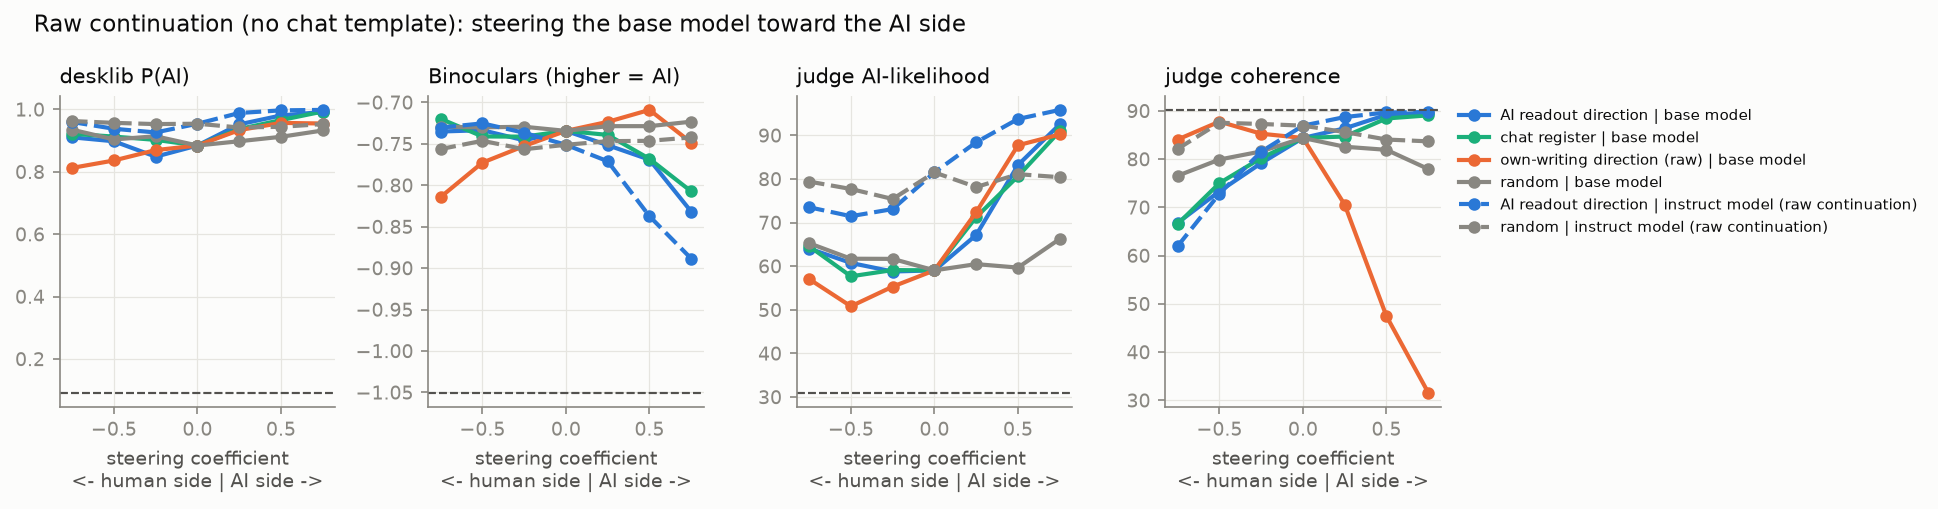
\includegraphics[width=\linewidth]{figures/fig5_base_model.png}
\caption{Steering raw continuation (150 \hape prefixes, no chat template). Adding the AI readout or chat-register direction to the base model raises the judge's AI-likelihood to the level of chat-model output while judged coherence rises. Random directions do not. Dashed horizontal lines mark human continuations.}
\label{fig:base}
\end{figure}

\begin{table}[t]
\centering
\caption{Steering raw continuation in the base and instruct models (150 \hape prefixes). \desklib and \bino are near ceiling here, so the result rests on the judge.}
\label{tab:basecont}
\resizebox{\textwidth}{!}{
\begin{tabular}{@{}llrccccccc@{}}
\toprule
Model & Condition & $c$ & Judge AI & \desklib & \bino flag & Coher. & On-task & Dist-3 & Readback \\
\midrule
-- & Human continuation & & 31.0 & 0.092 & 5 & 90.2 & 96.3 & 0.99 & 0.12 \\
\midrule
Base & Unsteered & & 59.0 & 0.884 & 97 & 84.4 & 87.0 & 0.86 & 0.82 \\
Base & \airead & $+0.25$ & 67.2 & 0.952 & 95 & 86.4 & 86.2 & 0.92 & 1.56 \\
Base & \airead & $+0.50$ & 83.2 & 0.981 & 95 & 89.2 & 81.6 & 0.95 & 2.99 \\
Base & \airead & $+0.75$ & {\bf 92.5} & 0.992 & 89 & {\bf 89.6} & 71.7 & 0.98 & 5.71 \\
Base & \chatreg & $+0.75$ & 91.0 & 0.993 & 97 & 89.1 & 73.7 & 0.97 & 4.80 \\
Base & \dir{random0} / \dir{random1} & $+0.75$ & 67.4 / 65.1 & 0.942 / 0.923 & 98 / 99 & 76.5 / 79.4 & 81.0 / 83.7 & 0.79 / 0.85 & 0.93 / 0.80 \\
Base & \airead & $-0.50$ & 60.7 & 0.898 & 95 & 73.3 & 78.0 & 0.76 & 0.17 \\
Base & \writeraw & $-0.50$ & 50.8 & 0.836 & 97 & 87.8 & 91.3 & 0.94 & 0.64 \\
Base & \writeraw & $+0.50$ & 87.7 & 0.957 & 91 & 47.4 & 55.4 & 0.45 & 0.36 \\
\midrule
Instruct & Unsteered & & 81.5 & 0.954 & 97 & 86.9 & 84.7 & 0.91 & 1.79 \\
Instruct & \airead & $+0.50$ & 93.8 & 0.997 & 93 & 89.7 & 74.5 & 0.98 & 4.36 \\
Instruct & \airead & $-0.50$ & 71.5 & 0.938 & 98 & 72.8 & 78.2 & 0.75 & 0.43 \\
\bottomrule
\end{tabular}}
\end{table}

\para{Steering the base model.}
\Figref{fig:base} and \tabref{tab:basecont} show that adding the direction to the base model raises the judge's AI-likelihood from 59.0 to 92.5 at $c=+0.75$: 26.3 points over random (Holm $p<0.001$), and 23.5 at $c=+0.5$.
Judged coherence {\em rises} ($+7$ to $+12$ over random) and repetition falls.
The base model starts writing in chat-model register.
Subtracting the direction does nothing to the judge, since the base model is already near the human position, and costs coherence.
The base model's own-writing direction (\writeraw, cosine 0.17 with \airead) is a different thing: adding it produces repetition collapse (distinct-3 0.45, external NLL 1.13), and subtracting it raises NLL and coherence and lowers the judge by 11 points over random.
H4 is supported.

\para{An unexpected baseline.}
Unsteered base-model continuations are flagged by \desklib (92\%) and \bino (97\%), unlike the 97--99\% ``human'' rates that \citet{xu2026base} report for GPTZero and Pangram.
Our continuations were sampled at temperature 0.7 and are repetitive (distinct-3 0.86; external NLL 1.80 vs.\ 2.87 for human text), whereas \citet{xu2026base} sample at temperature 1.0.
We did not rerun at 1.0, so the cause is not established.
